\documentclass{standalone}
\usepackage{pgfplots}
\pgfplotsset{compat=1.18}

\usetikzlibrary{calc}
\begin{document}
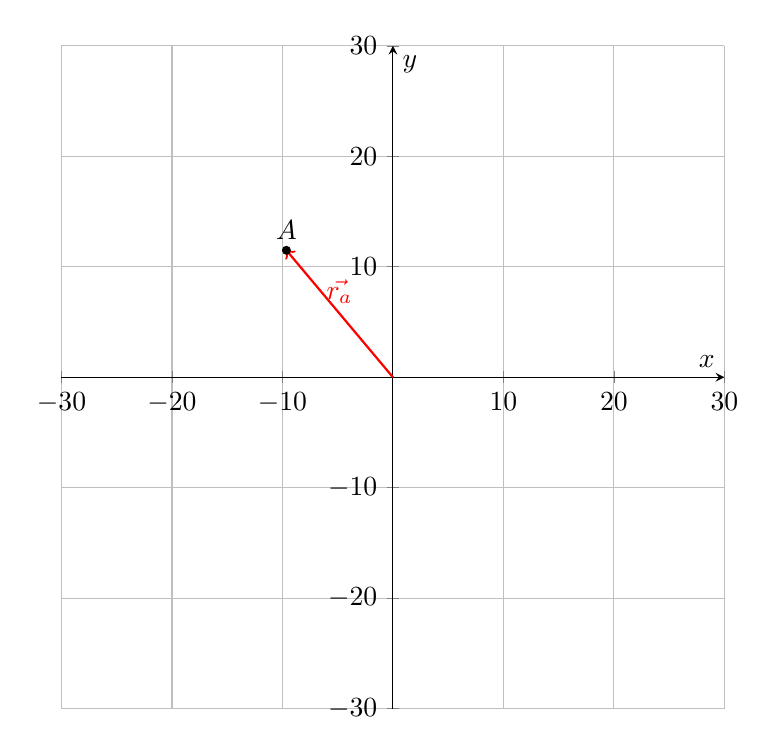
\begin{tikzpicture}
\begin{axis}[
  axis lines=middle,
  axis equal image,
  xlabel={$x$},
  ylabel={$y$},
  grid=both,
  xmin=-30,xmax=30,
  ymin=-30,ymax=30,
  width=10cm,
  height=10cm,
  ]

\coordinate (O) at (0,0);
\coordinate (A) at (130:15);

% \coordinate (C) at (130:15);


\draw[->, thick, red] (O) -- (A) node[midway, above] {$\vec{r_a}$};
\draw [->, thick, fill=black] (A) circle (0.3) node[above] {$A$};

\end{axis}
\end{tikzpicture}
\end{document}
